\hyt{scarboroughfaircarthy}
\song{Scarborough Fair}
\sub{Martin Carthy}
\hyl{scarboroughfair}{verze Simona \& Garfunkela}

\hspace{9mm}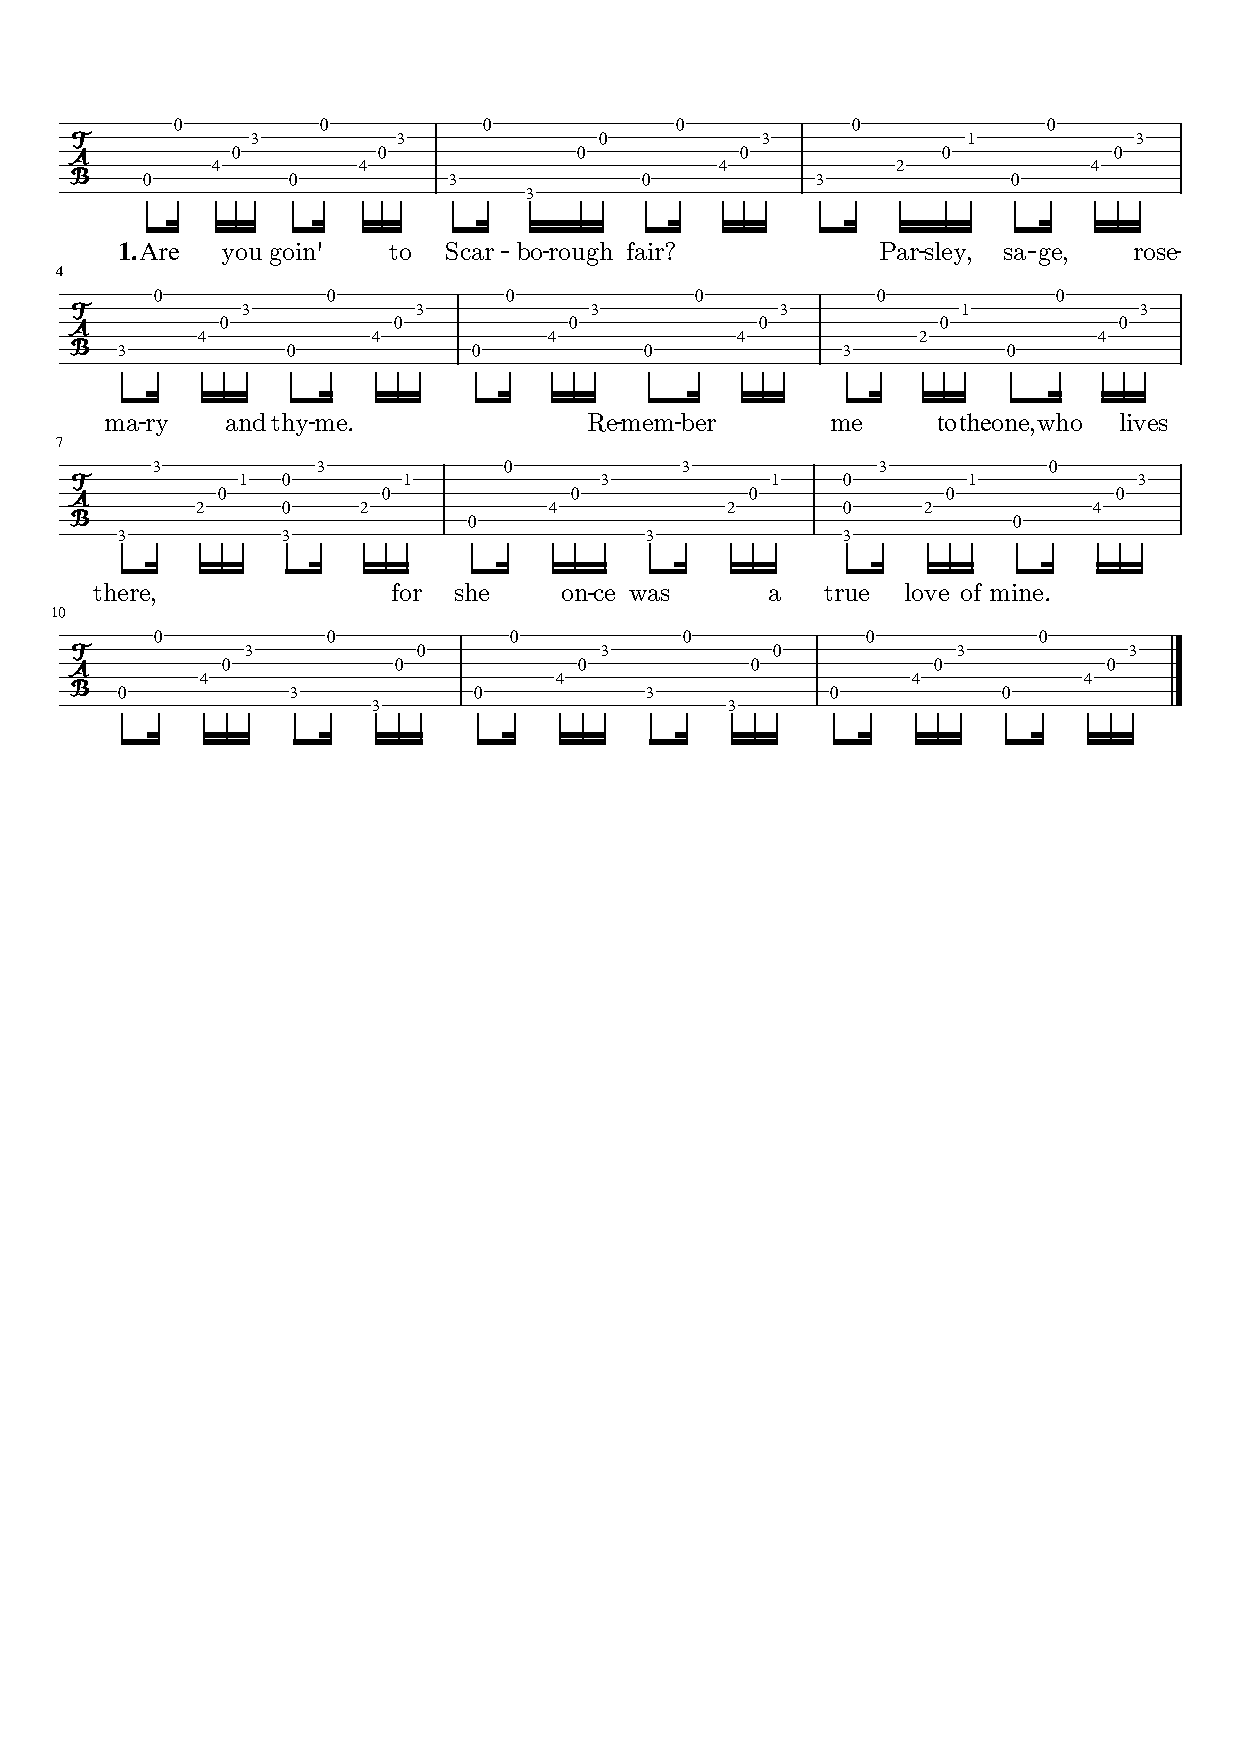
\includegraphics[width=0.99\linewidth]{scores/scarboroughfaircarthy.pdf}
\ns

\vers{2}{
Tell her to make me a cambric shirt.\\
Parsley, sage, rosemary and thyme.\\
Without no seam noe needlework\\
and then she'll be a true love of mine.
}	

\vers{3}{
Tell her to find me an acre of land.\\
Parsley, sage, rosemary and thyme.\\
Between the salt water and the sea strand\\
and then she'll be a true love of mine.
}

\vers{4}{
Tell her to plough it with a lamb's horn.\\
Parsley, sage, rosemary and thyme.\\
And to sow it all o'er with one peppercorn\\
and then she'll be a true love of mine.
}

\vers{5}{Tell her to reap it with a sickle of leather.\\
Parsley, sage, rosemary and thyme.\\
And to trash it all out with a bunch of heather\\
and then she'll be a true love of mine.
}

\vers{6}{
= \mm\textbf{1.}
}
	
\newpage
